%==============================================================================
%  STAT 5200 - Applied Econometrics I
%  Homework 1
%
%  Compile with:  pdflatex "HW 1 - Report.tex"  (run twice for refs)
%
%  Directory layout assumed by this file:
%     HW 1 - Report.tex
%     R/q1_matrix_algebra.R
%     R/q1_loop_sum.R
%     R/q2_monte_carlo.R
%     Figures/q2_hist_raw.pdf
%==============================================================================
\documentclass[11pt]{article}

\usepackage[margin=1in]{geometry}
\usepackage[T1]{fontenc}
\usepackage[utf8]{inputenc}
\usepackage{amsmath,amssymb}
\usepackage{booktabs}
\usepackage{graphicx}
\usepackage{xcolor}
\usepackage{listings}
\usepackage[font=small,labelfont=bf]{caption}
\usepackage[hidelinks]{hyperref}

%------------------------------------------------------------------------------
%  Code presentation
%
%  Conventions followed below (standard practice for code in academic reports):
%    * code is set as selectable text in a monospace font, never as a screenshot;
%    * every block is a captioned, labelled float-like object referred to by
%      number in the prose, so the text reads without the code;
%    * source code and program output use visually distinct styles, and are
%      never interleaved in the same block;
%    * Q1 shows its code in full directly under each question; Q2 shows short
%      excerpts in the body and its complete script in the appendix;
%    * the appendix listing is pulled from the .R file at compile time via
%      \lstinputlisting, so the report cannot drift from the code that was run;
%    * long lines wrap with a visible continuation marker instead of running
%      into the margin.
%------------------------------------------------------------------------------
\definecolor{codekeyword}{RGB}{0,86,148}
\definecolor{codestring} {RGB}{163,21,21}
\definecolor{codecomment}{RGB}{106,115,125}
\definecolor{codebg}     {RGB}{248,248,250}
\definecolor{coderule}   {RGB}{220,220,226}

\lstdefinestyle{Rcode}{
  language        = R,
  basicstyle      = \ttfamily\footnotesize,
  keywordstyle    = \color{codekeyword}\bfseries,
  stringstyle     = \color{codestring},
  commentstyle    = \color{codecomment}\itshape,
  numbers         = left,
  numberstyle     = \ttfamily\scriptsize\color{codecomment},
  numbersep       = 9pt,
  backgroundcolor = \color{codebg},
  frame           = single,
  rulecolor       = \color{coderule},
  framesep        = 4pt,
  xleftmargin     = 15pt,
  xrightmargin    = 0pt,
  % Fixed character grid: every glyph occupies exactly basewidth, so
  % indentation and aligned trailing comments line up down the block. With
  % fullflexible columns the glyphs take their natural widths instead, which
  % is what makes nominally aligned code drift out of line.
  columns         = fixed,
  basewidth       = 0.5em,
  keepspaces      = true,
  tabsize         = 2,
  showstringspaces = false,
  % Source lines are kept to 76 characters or fewer, which at \footnotesize on
  % a 0.5em grid needs about 342pt of the ~446pt available, so nothing wraps.
  % breaklines stays on only as a safety net; the marker should never appear.
  breaklines      = true,
  breakatwhitespace = true,
  postbreak       = \mbox{\textcolor{codekeyword}{$\hookrightarrow$}\space},
  captionpos      = b,
  abovecaptionskip = 6pt,
}

% Console output: same monospace face, but unhighlighted and unnumbered, so a
% reader can never mistake output for source.
\lstdefinestyle{Routput}{
  language        = {},          % no keyword highlighting for output
  basicstyle      = \ttfamily\footnotesize,
  keywordstyle    = \ttfamily,
  commentstyle    = \ttfamily,
  stringstyle     = \ttfamily,
  numbers         = none,
  backgroundcolor = \color{white},
  frame           = leftline,
  rulecolor       = \color{coderule},
  framesep        = 6pt,
  xleftmargin     = 20pt,
  breaklines      = true,
  captionpos      = b,
  abovecaptionskip = 6pt,
}

\lstset{style=Rcode}
\renewcommand{\lstlistingname}{Listing}

% Short inline code fragments.
\newcommand{\code}[1]{\texttt{#1}}

%------------------------------------------------------------------------------
\title{\vspace{-2em}Homework 1\\[0.3em]
       \large STAT 5200 --- Applied Econometrics I --- Fall 2026}

\author{Apostolos Kyratzis - 13130833}
\date{September 17, 2026}

\begin{document}
\maketitle

%==============================================================================
\section{Q1: Basic R questions}
%==============================================================================

\subsection{Matrix algebra}
\label{sec:q1-matrix}

\paragraph{(a) The two matrices.}
\[
A=\begin{pmatrix} 5 & 2\\ 2 & 1 \end{pmatrix},
\qquad
B=\begin{pmatrix} 5 & 2\\ 2 & 5 \end{pmatrix}
\]
Both are built with \code{matrix()}, using \code{byrow = TRUE} so that the
entries are typed row by row.

\begin{lstlisting}[style=Rcode]
A <- matrix(c(5, 2, 2, 1), nrow = 2, byrow = TRUE)
B <- matrix(c(5, 2, 2, 5), nrow = 2, byrow = TRUE)
\end{lstlisting}

\paragraph{(b) Computing $C = A^{-1}B$.}
\code{solve()} returns the inverse of a matrix and \code{\%*\%} is the matrix
product, so $C = A^{-1}B$ is computed as \code{solve(A) \%*\% B}.

\begin{lstlisting}[style=Rcode]
C <- solve(A) %*% B
print(C)
\end{lstlisting}

\begin{lstlisting}[style=Routput]
     [,1] [,2]
[1,]    1   -8
[2,]    0   21
\end{lstlisting}

\paragraph{(c) The transpose of $C$.}
\code{t()} transposes a matrix.

\begin{lstlisting}[style=Rcode]
print(t(C))
\end{lstlisting}

\begin{lstlisting}[style=Routput]
     [,1] [,2]
[1,]    1    0
[2,]   -8   21
\end{lstlisting}

\paragraph{(d) The difference between \texttt{A \%*\% B} and \texttt{A * B}.}
\code{\%*\%} is the matrix product: it combines rows of \code{A} with columns of
\code{B}, and requires \code{ncol(A) == nrow(B)}. \code{*} is the element-wise
product: it multiplies the entries in matching positions, and requires the two
matrices to have the same shape.

\begin{lstlisting}[style=Rcode]
print(A %*% B)
print(A * B)
\end{lstlisting}

\begin{lstlisting}[style=Routput]
     [,1] [,2]
[1,]   29   20
[2,]   12    9
     [,1] [,2]
[1,]   25    4
[2,]    4    5
\end{lstlisting}

\subsection{Matrix sum with a \texttt{for} loop}
\label{sec:q1-loop}

\[
X = \sum_{k=1}^{100} D_k,
\qquad
D_k = \begin{pmatrix} k & k+1\\ k^2 & k/2 \end{pmatrix}
\]
\code{X} starts as a $2\times2$ matrix of zeros from \code{matrix(0, nrow = 2,
ncol = 2)}, and each \code{D\_k} is added to it inside a \code{for} loop.

\begin{lstlisting}[style=Rcode]
X <- matrix(0, nrow = 2, ncol = 2)

for (k in 1:100) {
  D_k <- matrix(c(k, k + 1, k^2, k / 2), nrow = 2, byrow = TRUE)
  X <- X + D_k
}

print(X)
\end{lstlisting}

\begin{lstlisting}[style=Routput]
       [,1] [,2]
[1,]   5050 5150
[2,] 338350 2525
\end{lstlisting}

%==============================================================================
\section{Q2: Monte Carlo simulation (Lab Notes 01 quiz)}
\label{sec:q2}
%==============================================================================

\subsection{Setup}

The population model is
\[
y = \beta_0 + \beta_1 x + \beta_2 x^2 + \varepsilon,
\qquad
\beta_0 = 1,\; \beta_1 = 1,\; \beta_2 = 0.2,
\qquad
x \sim N(1, 4),
\]
and the object of interest is $\theta_0 = E[y]$, estimated by the sample mean
$\hat\theta = N^{-1}\sum_{i=1}^{N} y_i$.

The quiz replaces the original error distribution $\varepsilon \sim t_{10}$ with
\[
\varepsilon = v - 20, \qquad v \sim \chi^2(20).
\]
Since $E[v] = 20$, the new error still has mean zero, so the population object
of interest is unchanged at $\theta_0 = E[y] = 3$. What changes is the error
variance.

For a $t$ distribution with $\nu$ degrees of freedom the variance is
$\nu / (\nu - 2)$, defined for $\nu > 2$. With $\nu = 10$,
\[
\operatorname{Var}(\varepsilon) = \operatorname{Var}(t_{10})
 = \frac{\nu}{\nu - 2} = \frac{10}{10 - 2} = \frac{10}{8} = 1.25 .
\]

For a chi-squared distribution with $k$ degrees of freedom the variance is
$2k$. Subtracting the constant $20$ shifts the distribution without changing
its spread, so with $k = 20$,
\[
\operatorname{Var}(\varepsilon) = \operatorname{Var}(v - 20)
 = \operatorname{Var}(v) = 2k = 2 \times 20 = 40 .
\]

The error variance of the quiz model is therefore $40 / 1.25 = 32$ times that
of the original model.

The two errors also differ in shape. A $t$ distribution is symmetric about
zero, whereas a chi-squared distribution is right-skewed, and subtracting $20$
shifts it without removing that asymmetry. So the quiz model changes both the
spread and the shape of the error.

\subsection{Implementation}

The code follows Lab Notes 01. The lab's \code{generate\_data()} is renamed
\code{generate\_data\_t\_error()} and left otherwise untouched, and an identical
copy named \code{generate\_data\_x\_squared\_error()} is added in which the one
changed line draws the error from a recentred chi-squared distribution
(Listing~\ref{lst:q2-dgp}). Recentring at $v - 20$ is what preserves
$E[\varepsilon] = 0$, and hence $E[y] = 3$, across the two populations.

\begin{lstlisting}[style=Rcode,caption={The two data generating processes. Only
the line drawing \code{e} differs (excerpt from
\code{R/q2\_monte\_carlo.R}).},label={lst:q2-dgp}]
generate_data_t_error = function(N = 20){
  # model parameters
  beta0 = 1;
  beta1 = 1;
  beta2 = 0.2;
  # simulating data
  mat_data = matrix(NA, N, 2); # N by 2 matrix to store (y,x) by row
  for (i in 1:N){
    e = rt(1, df=10); # e ~ t distribution with degrees of freedom 10
    x = rnorm(1, mean=1, sd = sqrt(4)); # x~N(1,4)
    y = beta0 + beta1*x + beta2*x^2 + e; # this is our population model
    mat_data[i,] = c(y,x);
  }
  colnames(mat_data) = c("y", "x"); # put column names
  return(mat_data);
}

generate_data_x_squared_error = function(N = 20){
  # ... identical, except for the error term:
    e = rchisq(1, df=20) - 20; # e = v-20, v ~ chi-squared with df 20
}
\end{lstlisting}

The lab's \code{simulation\_sample\_mean()} is likewise duplicated, once per
population, each copy calling its own generator
(Listing~\ref{lst:q2-mc}). For a given $N$ it generates $M = 1000$ data sets,
computes the sample mean of $y$ in each, and returns the $M$ estimates.

\begin{lstlisting}[style=Rcode,caption={The Monte Carlo loop, duplicated once
per population (excerpt from \code{R/q2\_monte\_carlo.R}).},label={lst:q2-mc}]
simulation_sample_mean_t_error = function(N=20, M=1000){
  mat_theta_hat = matrix(NA, M, 1); # placeholder for M sample means
  for (m in 1:M){
    dataset = generate_data_t_error(N); # a data set (y,x) of length N
    theta_hat = mean(dataset[,1]); # compute sample mean of y
    mat_theta_hat[m,] = theta_hat; # store m-th sample mean
  }
  return(mat_theta_hat);
}

simulation_sample_mean_x_squared_error = function(N=20, M=1000){
  # ... identical, except that it calls
    dataset = generate_data_x_squared_error(N);
}
\end{lstlisting}

The $M$ estimates are collected into one matrix per population, with one column
per value of $N$, so that each half of the quiz is answered by reading across
the columns of a single object (Listing~\ref{lst:q2-collect}).

\begin{lstlisting}[style=Rcode,caption={Collecting the results, one matrix per
error distribution (excerpt from
\code{R/q2\_monte\_carlo.R}).},label={lst:q2-collect}]
M = 1000; # the number of simulations
N_grid = c(20, 100, 500); # the lengths of the data sets

mat_theta_hat_t_error = cbind(
  simulation_sample_mean_t_error(N = N_grid[1], M),
  simulation_sample_mean_t_error(N = N_grid[2], M),
  simulation_sample_mean_t_error(N = N_grid[3], M));

col_labels = c("N=20", "N=100", "N=500");
colnames(mat_theta_hat_t_error) = col_labels;

print(apply(mat_theta_hat_t_error, 2, var));

print(c("N=20"  = var(sqrt(20) *mat_theta_hat_t_error[,1]),
        "N=100" = var(sqrt(100)*mat_theta_hat_t_error[,2]),
        "N=500" = var(sqrt(500)*mat_theta_hat_t_error[,3])));
\end{lstlisting}

\subsection{Results}

Table~\ref{tab:q2} collects the Monte Carlo results.

\begin{table}[htbp]
\centering
\caption{Monte Carlo properties of the sample mean, $M = 1000$ replications,
$\theta_0 = 3$.}
\label{tab:q2}
\small
\begin{tabular}{llrrr}
\toprule
Error specification & $N$ & mean$(\hat\theta)$ &
$\operatorname{Var}(\hat\theta)$ &
$\operatorname{Var}(\sqrt{N}\hat\theta)$ \\
\midrule
$\varepsilon \sim t_{10}$ (original)
  & 20  & 2.965 & 0.5044 & 10.089 \\
  & 100 & 2.988 & 0.0972 &  9.716 \\
  & 500 & 3.000 & 0.0206 & 10.300 \\
\addlinespace
$\varepsilon = v - 20$, $v \sim \chi^2(20)$ (quiz)
  & 20  & 3.038 & 2.5436 & 50.871 \\
  & 100 & 3.001 & 0.4679 & 46.789 \\
  & 500 & 2.992 & 0.0977 & 48.853 \\
\bottomrule
\end{tabular}
\end{table}

\paragraph{Do we reach the same conclusion under the new population model?}
Yes --- every qualitative conclusion of the lab notes carries over, and only the
scale of the sampling uncertainty changes.

\begin{enumerate}
\item \emph{The estimator remains centred on $\theta_0 = 3$.} The Monte Carlo
means are $3.038$, $3.001$ and $2.992$, consistent with $\hat\theta$ being
unbiased. This is expected, because recentring the $\chi^2(20)$ draws at
$v - 20$ preserves $E[\varepsilon] = 0$ and hence leaves $E[y] = 3$ intact.

\item \emph{$\operatorname{Var}(\hat\theta)$ still falls at rate $1/N$.} Moving
from $N = 20$ to $N = 100$ divides the variance by $2.5436 / 0.4679 = 5.44$, and
moving from $N = 100$ to $N = 500$ divides it by $0.4679 / 0.0977 = 4.79$. Both
are close to the factor of $5$ by which $N$ was increased; the departures are
Monte Carlo noise from using only $M = 1000$ replications.

\item \emph{$\operatorname{Var}(\sqrt{N}\hat\theta)$ does not shrink with $N$.}
The values $50.87$, $46.79$ and $48.85$ show no trend, just as $10.089$,
$9.716$ and $10.300$ do not in the original model.
\end{enumerate}

The only difference is the \emph{level}: sampling uncertainty is about four to
five times larger throughout. That is a smaller increase than the $32$-fold
rise in $\operatorname{Var}(\varepsilon)$, because the error is only one
component of $\operatorname{Var}(y)$: the contribution of $x$ is the same in
both populations, so only part of the variance changes.

\paragraph{Histograms of $\sqrt{N}\hat\theta$ at $N = 500$.}
Figure~\ref{fig:q2-raw} plots the two simulated distributions on a common
horizontal axis. Both are single-peaked, symmetric and centred on
$\sqrt{500} \times 3 \approx 67.08$, but the $\chi^2$ case is visibly wider,
which is the variance difference of Table~\ref{tab:q2} seen directly.

\begin{figure}[htbp]
\centering
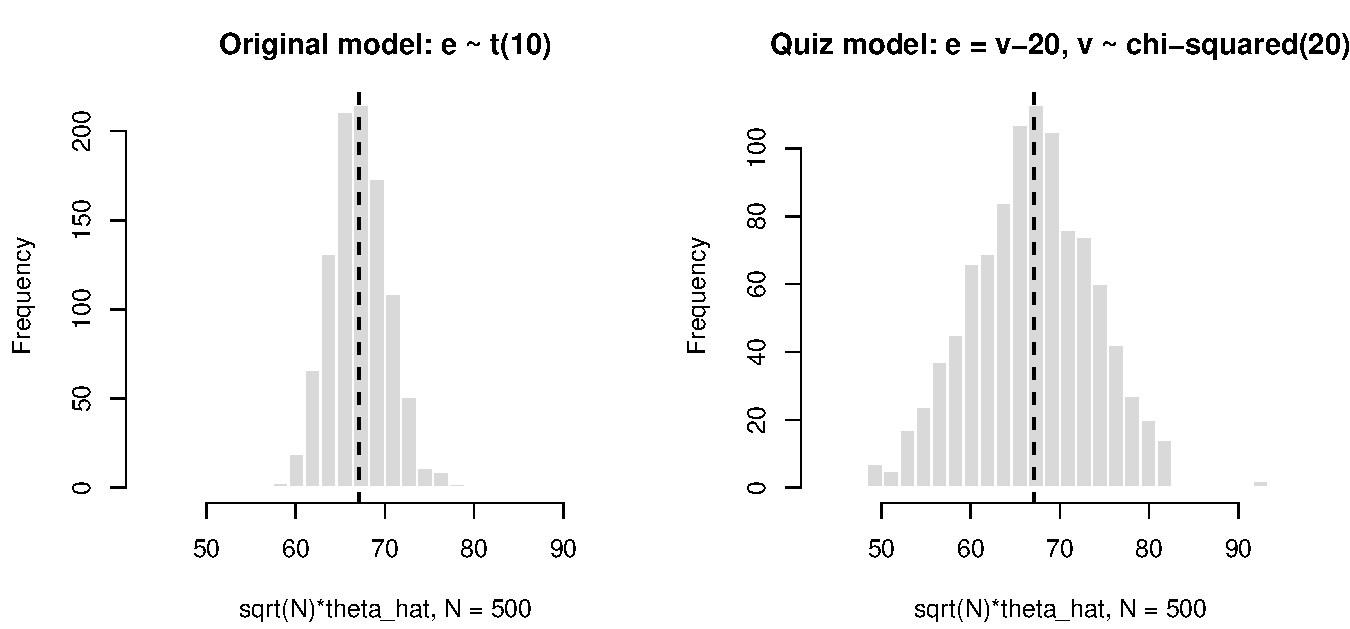
\includegraphics[width=\textwidth]{Figures/q2_hist_raw.pdf}
\caption{Simulated distribution of $\sqrt{N}\hat\theta$ at $N = 500$,
$M = 1000$, on a common horizontal axis. The dashed line marks
$\sqrt{N}\theta_0 \approx 67.08$. Left: original $t_{10}$ errors. Right: the
quiz model, $\varepsilon = v - 20$ with $v \sim \chi^2(20)$.}
\label{fig:q2-raw}
\end{figure}

So the answer is: \emph{yes, they look similar} --- both are bell-shaped and
centred on the same point, and differ only in width. This is worth remarking on,
because the two errors are not similar: one is symmetric and the other
right-skewed. It is what the central limit theorem leads us to expect, though,
since an average of many observations is approximately normal whatever the shape
of the distribution being averaged. Averaging $N = 500$ observations is enough
to leave no visible trace of the skewness of the $\chi^2$ error.

%==============================================================================
\section{Q3: Paper questions}
%==============================================================================

\paragraph{(1) Field of interest.}
Operations Management.

\paragraph{(2) Five well-read journals in the field.}
\begin{enumerate}
\item \emph{Management Science}
\item \emph{Operations Research}
\item \emph{Manufacturing \& Service Operations Management}
\item \emph{Production and Operations Management}
\item \emph{Journal of Operations Management}
\end{enumerate}

\paragraph{(3) The paper.}
I chose \emph{Market Fragmentation and Inefficiencies in Maritime Shipping},
by Bimpikis, Mantegazza and Wollenstein-Betech. It contains the word
``econometric'' (its Appendix~B is titled ``Econometric details''), it applies
econometric methods to data (its Sections 3.4, 4.2 and 4.3), and it presents
results from that analysis (its Tables 5--13).

I acknowledge that it is not published in one of the five journals listed
above. It appeared in the proceedings of the ACM Conference on Economics and
Computation, which is a peer-reviewed conference rather than a journal. I chose
it anyway because I read it recently for a research project, I find it genuinely
interesting, and it leaves open a number of directions for follow-up research
--- among them endogenising transportation demand rather than holding it fixed,
estimating a structural model once data on contracted rates are available, and
studying how operational coordination interacts with carbon pricing.

\paragraph{(4) Citation.}
Bimpikis, K., Mantegazza, G., and Wollenstein-Betech, S. (2024). Market
fragmentation and inefficiencies in maritime shipping. In \emph{Proceedings of
the 25th ACM Conference on Economics and Computation (EC~'24)}. Association for
Computing Machinery. \url{https://doi.org/10.1145/3670865.3673494}

Bimpikis, K., Mantegazza, G., and Wollenstein-Betech, S. (2025). Market
fragmentation and inefficiencies in maritime shipping. \emph{SSRN Working
Paper No.~6560678}.

\paragraph{(5) The main research question.}
Roughly half of all miles travelled by oil tankers are sailed empty, a practice
known as ballasting, and the paper asks how much of that waste is actually
avoidable. Some of it is not: oil is produced in a few places and consumed in
many, so geographic trade imbalances force vessels to reposition without cargo,
and operators must commit to those moves before knowing when or where the next
cargo will appear. The authors ask what remains once those two forces are
accounted for, and attribute the remainder to \emph{market fragmentation} ---
the fact that no single commercial operator controls more than about 5\% of
global tanker capacity, so each optimises over its own small fleet and cannot
internalise the repositioning externalities it imposes on the others. They call
this residual the \emph{fragmentation tax}. The distinction matters because the
two components differ in what policy can do about them: geography is fixed,
whereas fragmentation is a feature of how the industry is organised and could in
principle be changed without any new technology. The paper then asks the
natural follow-up question of how much consolidation (via vessel pooling) would be needed to recover those losses, and whether shipping pools can deliver it without conferring
market power.

\paragraph{(6) The econometric method used.}
The main method is \emph{instrumental variables estimation by two-stage least
squares} on a panel with two-way fixed effects. The components are:

\begin{itemize}
\item ordinary least squares with two-way fixed effects, as a baseline;
\item two-stage least squares, for the endogenous regressors (market
concentration, measured by the Herfindahl--Hirschman index, and pool size);
\item a lagged instrument, instrumenting concentration by its own one-quarter
lag;
\item Hausman-style instruments, built from peer-group average fleet size;
\item log-log specifications, so that coefficients read as elasticities;
\item first-stage $F$ and Wald statistics, as weak-instrument diagnostics.
\end{itemize}

The rest of the paper uses integer linear programming and approximate dynamic
programming. Those are methods of operations research rather than
econometrics, and the authors present the regressions above as independent
validation of the results they obtain from them.

\paragraph{(7) Do the authors report standard errors?}
Yes, for every regression. They appear in parentheses beneath each coefficient,
together with significance stars, and they are clustered rather than
conventional. Table~\ref{tab:q3-table5} reproduces the paper's Table~5, which
is the regression that validates its central claim: markets in which vessel
control is more concentrated ballast shorter distances, emit less, and spend
less time empty. The authors also report first-stage Wald statistics, and
elsewhere use them to flag one of their alternative instruments as weak.

\begin{table}[htbp]
\centering
\caption{Table~5 of Bimpikis et al., reproduced. Market-level regressions of
ballast efficiency measures on market concentration, measured by the
Herfindahl--Hirschman index. The instrument in the IV columns is
$\log(\mathrm{HHI}_{l,v,t-1})$. Clustered standard errors in parentheses;
significance codes ${}^{***}\,0.01$, ${}^{**}\,0.05$, ${}^{*}\,0.1$.}
\label{tab:q3-table5}
\footnotesize
\setlength{\tabcolsep}{4pt}
\begin{tabular}{lrrrrrr}
\toprule
& \multicolumn{2}{c}{Ballast distance (nm)}
& \multicolumn{2}{c}{Ballast emissions (CO$_2$)}
& \multicolumn{2}{c}{Ballast time (days)} \\
\cmidrule(lr){2-3} \cmidrule(lr){4-5} \cmidrule(lr){6-7}
& OLS & IV & OLS & IV & OLS & IV \\
\midrule
$\log(\mathrm{HHI})$
  & $-0.2581^{***}$ & $-0.3229^{***}$
  & $-0.2428^{***}$ & $-0.3039^{***}$
  & $-0.2026^{***}$ & $-0.2434^{***}$ \\
  & $(0.0543)$ & $(0.0667)$
  & $(0.0461)$ & $(0.0591)$
  & $(0.0458)$ & $(0.0527)$ \\
\addlinespace
\multicolumn{7}{l}{\emph{Fixed effects}} \\
\quad Load area & Yes & Yes & Yes & Yes & Yes & Yes \\
\quad Quarter   & Yes & Yes & Yes & Yes & Yes & Yes \\
\addlinespace
\multicolumn{7}{l}{\emph{Fit statistics}} \\
\quad Observations & 2{,}297 & 2{,}143 & 2{,}297 & 2{,}143
  & 2{,}297 & 2{,}143 \\
\quad $R^2$ & 0.90674 & 0.99175 & 0.94668 & 0.99397
  & 0.93063 & 0.99455 \\
\quad Wald (1st stage $F$) & --- & 100.85 & --- & 100.85
  & --- & 100.85 \\
\bottomrule
\end{tabular}
\end{table}

\paragraph{(8) What is a standard error? (not graded)}
The starting point, following Wooldridge, is that an estimator is a random
variable. We only ever see one sample, but that sample was drawn by chance, and
a different draw would have handed us a different number. How much the estimate
moves from sample to sample is captured by the standard deviation of the
estimator, which in the simple regression case is
\[
\operatorname{sd}(\hat\beta_1) = \frac{\sigma}{\sqrt{SST_x}},
\qquad
SST_x = \sum_{i=1}^{n}(x_i - \bar{x})^2 .
\]
The trouble is that we cannot compute this, because $\sigma$, the standard
deviation of the population error, is unknown.

The standard error is what we get by putting an estimate in its place:
\[
\operatorname{se}(\hat\beta_1) = \frac{\hat\sigma}{\sqrt{SST_x}} .
\]
So a standard error is an \emph{estimate of the standard deviation of an
estimator}. $\operatorname{sd}(\hat\beta_1)$ is a
population quantity we never observe, whereas $\operatorname{se}(\hat\beta_1)$
is computed from the data in front of us, and is therefore itself a random
variable. It is precisely because it can be computed that it can be printed
underneath a coefficient in Table~\ref{tab:q3-table5}, and that $t$ statistics
and confidence intervals can be built out of it.

%==============================================================================
\appendix
\section{Complete R scripts}
\label{app:code}
%==============================================================================

The listing in this appendix is read directly from the \code{.R} file at compile
time, so it is a verbatim copy of the code that produced the results above. The
Q1 scripts are not repeated here, since they appear in full alongside the
questions in Section~\ref{sec:q1-matrix} and Section~\ref{sec:q1-loop}.

\subsection{\texorpdfstring{\code{R/q2\_monte\_carlo.R}}{R/q2\_monte\_carlo.R}}
\lstinputlisting[style=Rcode,caption={\code{R/q2\_monte\_carlo.R} --- Q2, Monte
Carlo study of the sample mean under both error
specifications.},label={lst:app-q2}]{R/q2_monte_carlo.R}

\end{document}
